\documentclass{report}
%%%%%%%%%%%%%% preamble.tex %%%%%%%%%%%%%%
\usepackage[T1]{fontenc}
\usepackage{etoolbox}
% Page Setup
\usepackage[letterpaper, tmargin=2cm, rmargin=0.5in, lmargin=0.5in, bmargin=80pt, footskip=.2in]{geometry}
\usepackage{adjustbox}
\usepackage{graphicx}
\usepackage{tikz}
\usepackage{mathrsfs}
\usepackage{mdframed}

% Create a new toggle
\newtoggle{firstsection}

% Redefine the \chapter command to reset the toggle for each new chapter
\let\oldchapter\chapter
\renewcommand{\chapter}{\toggletrue{firstsection}\oldchapter}

% Redefine the \section command to check the toggle
\let\oldsection\section
\renewcommand{\section}{
    \iftoggle{firstsection}
    {\togglefalse{firstsection}} % If it's the first section, just switch off the toggle for next sections
    {\clearpage} % If it's not the first section, start a new page
    \oldsection
}

% Abstract Design

\usepackage{lipsum}

\renewenvironment{abstract}
 {% Start of environment
  \quotation
  \small
  \noindent
  \rule{\linewidth}{.5pt} % Draw the rule to match the linewidth
  \par\smallskip
  {\centering\bfseries\abstractname\par}\medskip
 }
 {% End of environment
  \par\noindent
  \rule{\linewidth}{.5pt} % Ensure the closing rule also matches
  \endquotation
 }

% Mathematics
\usepackage{amsmath,amsfonts,amsthm,amssymb,mathtools}
\usepackage{xfrac}
\usepackage[makeroom]{cancel}
\usepackage{enumitem}
\usepackage{nameref}
\usepackage{multicol,array}
\usepackage{tikz-cd}
\usepackage{array}
\usepackage{multirow}% http://ctan.org/pkg/multirow
\usepackage{graphicx}

% Colors
\usepackage[dvipsnames]{xcolor}
\definecolor{myg}{RGB}{56, 140, 70}
\definecolor{myb}{RGB}{45, 111, 177}
\definecolor{myr}{RGB}{199, 68, 64}
% Define more colors here...
\definecolor{olive}{HTML}{6B8E23}
\definecolor{orange}{HTML}{CC5500}
\definecolor{brown}{HTML}{8B4513}
% Hyperlinks
\usepackage{bookmark}
\usepackage[colorlinks=true,linkcolor=blue,urlcolor=blue,citecolor=blue,anchorcolor=blue]{hyperref}
\usepackage{xcolor}
\hypersetup{
    colorlinks,
    linkcolor={red!50!black},
    citecolor={blue!50!black},
    urlcolor={blue!80!black}
}

% Text-related
\usepackage{blindtext}
\usepackage{fontsize}
\changefontsize[14]{14}
\setlength{\parindent}{0pt}
\linespread{1.2}

% Theorems and Definitions
\usepackage{amsthm}
\renewcommand\qedsymbol{$\blacksquare$}

% Define a new theorem style
\newtheoremstyle{mytheoremstyle}% name
  {}% Space above
  {}% Space below
  {}% Body font
  {}% Indent amount
  {\bfseries}% Theorem head font
  {.}% Punctuation after theorem head
  {.5em}% Space after theorem head
  {}% Theorem head spec (can be left empty, meaning ‘normal’)

% Apply the new theorem style to theorem-like environments
\theoremstyle{mytheoremstyle}

\newtheorem{theorem}{Theorem}[section]  
\newtheorem{definition}[theorem]{Definition} 
\newtheorem{lemma}[theorem]{Lemma}  
\newtheorem{corollary}[theorem]{Corollary}
\newtheorem{axiom}[theorem]{Axiom}
\newtheorem{example}[theorem]{Example}
\newtheorem{equiv_def}[theorem]{Equivalent Definition}

% tcolorbox Setup
\usepackage[most,many,breakable]{tcolorbox}
\tcbuselibrary{theorems}

% Define custom tcolorbox environments here...

%================================
% EXAMPLE BOX
%================================
% After you have defined the style and other theorem environments
\definecolor{myexamplebg}{RGB}{245, 245, 245} % Very light grey for background
\definecolor{myexamplefr}{RGB}{120, 120, 120} % Medium grey for frame
\definecolor{myexampleti}{RGB}{60, 60, 60}    % Darker grey for title

\newtcbtheorem[]{Example}{Example}{
    colback=myexamplebg,
    breakable,
    colframe=myexamplefr,
    coltitle=myexampleti,
    boxrule=1pt,
    sharp corners,
    detach title,
    before upper=\tcbtitle\par\vspace{-20pt}, % Reduced the space after the title
    fonttitle=\bfseries,
    description font=\mdseries,
    separator sign none,
    description delimiters={}{}, % No delimiters around the title
}{ex}
%================================
% Solution BOX
%================================
\makeatletter
\newtcolorbox{solution}{enhanced,
	breakable,
	colback=white,
	colframe=myg!80!black,
	attach boxed title to top left={yshift*=-\tcboxedtitleheight},
	title=Solution,
	boxed title size=title,
	boxed title style={%
			sharp corners,
			rounded corners=northwest,
			colback=tcbcolframe,
			boxrule=0pt,
		},
	underlay boxed title={%
			\path[fill=tcbcolframe] (title.south west)--(title.south east)
			to[out=0, in=180] ([xshift=5mm]title.east)--
			(title.center-|frame.east)
			[rounded corners=\kvtcb@arc] |-
			(frame.north) -| cycle;
		},
}
\makeatother

% %================================
% % Question BOX
% %================================
\makeatletter
\newtcbtheorem{question}{Question}{enhanced,
	breakable,
	colback=white,
	colframe=myb!80!black,
	attach boxed title to top left={yshift*=-\tcboxedtitleheight},
	fonttitle=\bfseries,
	title={#2},
	boxed title size=title,
	boxed title style={%
			sharp corners,
			rounded corners=northwest,
			colback=tcbcolframe,
			boxrule=0pt,
		},
	underlay boxed title={%
			\path[fill=tcbcolframe] (title.south west)--(title.south east)
			to[out=0, in=180] ([xshift=5mm]title.east)--
			(title.center-|frame.east)
			[rounded corners=\kvtcb@arc] |-
			(frame.north) -| cycle;
		},
	#1
}{question}
\makeatother

%%%%%%%%%%%%%%%%%%%%%%%%%%%%%%%%%%%%%%%%%%%
% TABLE OF CONTENTS
%%%%%%%%%%%%%%%%%%%%%%%%%%%%%%%%%%%%%%%%%%%


\usepackage{tikz}
\definecolor{doc}{RGB}{0,60,110}
\usepackage{titletoc}
\contentsmargin{0cm}
\titlecontents{chapter}[14pc]
{\addvspace{30pt}%
	\begin{tikzpicture}[remember picture, overlay]%
		\draw[fill=doc!60,draw=doc!60] (-7,-.1) rectangle (-0.9,.5);%
		\pgftext[left,x=-5.5cm,y=0.2cm]{\color{white}\Large\sc\bfseries Chapter\ \thecontentslabel};%
	\end{tikzpicture}\color{doc!60}\large\sc\bfseries}%
{}
{}
{\;\titlerule\;\large\sc\bfseries Page \thecontentspage
	\begin{tikzpicture}[remember picture, overlay]
		\draw[fill=doc!60,draw=doc!60] (2pt,0) rectangle (4,0.1pt);
	\end{tikzpicture}}%
\titlecontents{section}[3.7pc]
{\addvspace{2pt}}
{\contentslabel[\thecontentslabel]{3pc}}
{}
{\hfill\small \thecontentspage}
[]
\titlecontents*{subsection}[3.7pc]
{\addvspace{-1pt}\small}
{}
{}
{\ --- \small\thecontentspage}
[ \textbullet\ ][]

\makeatletter
\renewcommand{\tableofcontents}{
	\chapter*{%
	  \vspace*{-20\p@}%
	  \begin{tikzpicture}[remember picture, overlay]%
		  \pgftext[right,x=15cm,y=0.2cm]{\color{doc!60}\Huge\sc\bfseries \contentsname};%
		  \draw[fill=doc!60,draw=doc!60] (13,-.75) rectangle (20,1);%
		  \clip (13,-.75) rectangle (20,1);
		  \pgftext[right,x=15cm,y=0.2cm]{\color{white}\Huge\sc\bfseries \contentsname};%
	  \end{tikzpicture}}%
	\@starttoc{toc}}
\makeatother

\newcommand{\liff}{\llap{$\iff$}}
\newcommand{\rap}[1]{\rrap{\text{ (#1)}}}
\newcommand{\red}[1]{\textcolor{red}{#1}}
\newcommand{\blue}[1]{\textcolor{blue}{#1}}
\newcommand{\vi}[1]{\textcolor{violet}{#1}}
\newcommand{\olive}[1]{\textcolor{olive}{#1}}
\newcommand{\teal}[1]{\textcolor{teal}{#1}}
\newcommand{\brown}[1]{\textcolor{brown}{#1}}
\newcommand{\orange}[1]{\textcolor{orange}{#1}}
\newcommand{\tCaC}{\text{ \CaC }}
\newcommand{\CaC}{\red{CaC} }
\newcommand{\As}[1]{Assume \red{#1}}
\newcommand{\vdone}{\vi{\text{ (done) }}}
\newcommand{\bdone}{\blue{\text{ (done) }}}
\newcommand{\tdone}{\teal{\text{ (done) }}}
\newcommand{\odone}{\olive{\text{ (done) }}}
\newcommand{\bodone}{\brown{\text{ (done) }}}
\newcommand{\ordone}{\orange{\text{ (done) }}}
\newcommand{\ld}{\lambda}
\newcommand{\vecta}[1]{\textbf{#1}}
\newcommand{\set}[1]{\left\{ #1 \right\}}
\newcommand{\bset}[1]{\Big\{ #1 \Big\}}
\newcommand{\inR}{\in\R}
\newcommand{\inn}{\in\N}
\newcommand{\inz}{\in\Z}
\newcommand{\inr}{\in\R}
\newcommand{\inc}{\in\C}
\newcommand{\inq}{\in\Q}
\newcommand{\norm}[1]{\| #1 \|}
\newcommand{\bnorm}[1]{\Big\| #1 \Big\|}
\newcommand{\gen}[1]{\langle #1 \rangle}
\newcommand{\abso}[1]{\left|#1\right|}
\newcommand{\myref}[2]{\hyperref[#2]{#1\ \ref*{#2}}}
\newcommand{\customref}[2]{\hyperref[#1]{#2}}
\newcommand{\power}[1]{\mathcal{P}(#1)}
\newcommand{\dcup}{\mathbin{\dot{\cup}}}
\newcommand{\diam}[1]{\text{diam}\, #1}
\newcommand{\at}{\Big|}
\newcommand{\quotient}{\diagup}
\let\originalphi\phi % Store the original \phi in \originalphi
\renewcommand{\phi}{\varphi} % Redefine \phi to \varphi
\newcommand{\pfi}{\originalphi} % Define \pfi to display the original \phi
\newcommand{\diota}{\dot{\iota}}
\newcommand{\Log}{\operatorname{Log}}
\newcommand{\id}{\text{\textbf{id}}}
\usepackage{amsmath}

\makeatletter
\NewDocumentCommand{\extp}{e{^}}{%
  \mathop{\mathpalette\extp@{#1}}\nolimits
}
\NewDocumentCommand{\extp@}{mm}{%
  \bigwedge\nolimits\IfValueT{#2}{^{\extp@@{#1}#2}}%
  \IfValueT{#1}{\kern-2\scriptspace\nonscript\kern2\scriptspace}%
}
\newcommand{\extp@@}[1]{%
  \mkern
    \ifx#1\displaystyle-1.8\else
    \ifx#1\textstyle-1\else
    \ifx#1\scriptstyle-1\else
    -0.5\fi\fi\fi
  \thinmuskip
}
\makeatletter
\usepackage{pifont}
\makeatletter
\newcommand\Pimathsymbol[3][\mathord]{%
  #1{\@Pimathsymbol{#2}{#3}}}
\def\@Pimathsymbol#1#2{\mathchoice
  {\@Pim@thsymbol{#1}{#2}\tf@size}
  {\@Pim@thsymbol{#1}{#2}\tf@size}
  {\@Pim@thsymbol{#1}{#2}\sf@size}
  {\@Pim@thsymbol{#1}{#2}\ssf@size}}
\def\@Pim@thsymbol#1#2#3{%
  \mbox{\fontsize{#3}{#3}\Pisymbol{#1}{#2}}}
\makeatother
% the next two lines are needed to avoid LaTeX substituting upright from another font
\input{utxmia.fd}
\DeclareFontShape{U}{txmia}{m}{n}{<->ssub * txmia/m/it}{}
% you may also want
\DeclareFontShape{U}{txmia}{bx}{n}{<->ssub * txmia/bx/it}{}
% just in case
%\DeclareFontShape{U}{txmia}{l}{n}{<->ssub * txmia/l/it}{}
%\DeclareFontShape{U}{txmia}{b}{n}{<->ssub * txmia/b/it}{}
% plus info from Alan Munn at https://tex.stackexchange.com/questions/290165/how-do-i-get-a-nicer-lambda?noredirect=1#comment702120_290165
\newcommand{\pilambdaup}{\Pimathsymbol[\mathord]{txmia}{21}}
\renewcommand{\lambda}{\pilambdaup}
\renewcommand{\tilde}{\widetilde}
\DeclareMathOperator*{\esssup}{ess\,sup}
\newcommand{\bluecheck}{}%
\DeclareRobustCommand{\bluecheck}{%
  \tikz\fill[scale=0.4, color=blue]
  (0,.35) -- (.25,0) -- (1,.7) -- (.25,.15) -- cycle;%
}


\usepackage{tikz}
\newcommand*{\DashedArrow}[1][]{\mathbin{\tikz [baseline=-0.25ex,-latex, dashed,#1] \draw [#1] (0pt,0.5ex) -- (1.3em,0.5ex);}}

\newcommand{\C}{\mathbb{C}}	
\newcommand{\F}{\mathbb{F}}
\newcommand{\N}{\mathbb{N}}
\newcommand{\Q}{\mathbb{Q}}
\newcommand{\R}{\mathbb{R}}
\newcommand{\Z}{\mathbb{Z}}



\title{\Huge{NCKU 112.2}\\
Miscellaneous Facts}
\author{\huge{Eric Liu}}
\date{}
\begin{document}
\maketitle
\newpage% or \cleardoublepage
% \pdfbookmark[<level>]{<title>}{<dest>}
\pdfbookmark[section]{\contentsname}{toc}
\tableofcontents
\pagebreak

\chapter{General Topology}
\section{Directed Sets}
\begin{axiom}
\label{1.1.1}
\textbf{(Axioms in Order Theory)} Given an relation $(X,\leq )$, and suppose  $x,y,z \in X$. 
\begin{enumerate}[label=(\alph*)]
  \item $x\leq x$ (Reflexive)
  \item $x\leq y\leq z \implies x\leq z$ (Transitive)
  \item $x\leq y\text{ and }y\leq x\implies x=y$ (Antisymmetric)
  \item $x\leq y\text{ or }y\leq x$ (Connected)
  \item $\forall x,y \in X, \exists z\in X, x\leq z\text{ and }y\leq z$ (Directed)
\end{enumerate}
We say $(X,\leq )$ form a 
\begin{enumerate}[label=(\alph*)]
  \item \red{total order} if it is reflexive, transitive, antisymmetric and connected. 
  \item \red{partial order} if it is reflexive, transitive and  antisymmetric. 
  \item \red{preorder} if it is reflexive and transitive.
  \item \red{directed set} if it is reflexive, transitive and directed. 
\end{enumerate}
\end{axiom}
\begin{theorem}
\label{1.1.2}
\textbf{(Why is it called Preorder)} Given a preorder $(X,\leq )$, the relation $\sim$ defined by 
\begin{align*}
x\sim y \iff x\leq y\text{ and }y\leq x
\end{align*}
is an equivalence relation and if we define $\leq^e$ on the equivalence class by 
\begin{align*}
\exists x \in A, y \in B, x\leq y \implies A\leq^e B
\end{align*}
Then $\leq^e$ is a partial order. Moreover, if the preorder $\leq $ is directed, then $\leq ^e$ is also directed.
\end{theorem}
\begin{proof}
We first show \vi{$\sim$ is an equivalence relation}. Because preoder is reflexive, we see 
\begin{align*}
\forall x\in X, x\leq x\text{ which implies }\forall x \in X, x \sim x
\end{align*}
For symmetry, it is easy to see 
\begin{align*}
x\sim y \implies x\leq y\text{ and }y\leq x\implies y\sim x
\end{align*}
For transitive, see 
\begin{align*}
  x\sim y \text{ and } y\sim z&\implies x\leq y \text{ and }y \leq x \text{ and }y\leq z \text{ and }z \leq y \\
&\implies x\leq z\text{ and } z\leq x\implies x\sim z \vdone
\end{align*}
We now show \blue{$\leq^e$ is a partial order}. Reflexive property and Transitive property of $\leq^e$ follow from that of $\leq $. Suppose $A\leq^e B$ and $B\leq^e A$, where $x_1,x_2\in A,y_1,y_2\in B$ satisfy $x_1\leq y_1$ and $y_2\leq x_2$. Because $x_1,x_2 \in A$ and $y_1,y_2\in B$, we have 
\begin{align*}
x_1\leq x_2\text{ and }x_2\leq x_1\text{ and }y_1\leq y_2\text{ and }y_2\leq y_1
\end{align*}
Then because $\leq $ satisfy transitive, we have 
\begin{align*}
\begin{cases}
  x_2\leq x_1\leq y_1 \implies x_2\leq y_1\\
  y_1\leq y_2\leq x_2 \implies y_1\leq x_2
\end{cases}
\end{align*}
This tell us 
\begin{align*}
x_2 \sim y_1
\end{align*}
which implies $A=B$, thus proving  $\leq^e$ is antisymmetirc. $\bdone$\\

Lastly, we show  \vi{$\leq $ is directed$\implies \leq ^e$ is directed}. Let $A,B$ be two arbitrary equivalence class. We wish to find an equivalence class $T$ such that 
\begin{align*}
A\leq^e T \text{ and } B\leq^e T
\end{align*}
Let $a,b$ respectively be an arbitrary element of $A,B$. Because  $\leq $ is directed, we know there exists $c\in X$ such that 
\begin{align*}
a\leq c\text{ and }b\leq c
\end{align*}
We immediately see 
\begin{align*}
A\leq^e [c] \text{ and } B\leq^e [c] \vdone
\end{align*}
\end{proof}
\begin{corollary}
\label{1.1.3}
\textbf{(Chunk Structure of Preorder)} Given two equivalence class $A,B$, we have
 \begin{align*}
A\leq^e B \implies \forall x\in A,y \in B, x\leq y
\end{align*}
\end{corollary}
\begin{proof}
Because $A\leq ^e B$, we know 
\begin{align*}
\exists x_0\in A,y_0\in B, x_0\leq y_0
\end{align*}
Then by definition of $\sim$, we have
\begin{align*}
x \leq x_0\leq y_0\leq y
\end{align*}
This give us 
\begin{align*}
x\leq y
\end{align*}
\end{proof}
\begin{definition}
\label{1.1.4}
\textbf{(Definition of Maximal element in Preorder)} Let $(I,\leq )$ be a preorder. We say $m\in I$ is a maximal element if 
\begin{align*}
\forall y\in I, m\leq y\implies y\leq m
\end{align*}
\end{definition}
\begin{theorem}
\label{1.1.5}
\textbf{(In Preorder, Maximal element form an Equivalence class)} Let $(I,\leq )$ be a preorder, and $m \in  I$ be a maximal element. Then 
\begin{align*} 
\forall x\in [m], x\text{ is a maximal element }
\end{align*}
\end{theorem}
\begin{proof}
Arbitrarily pick an element $x$ in $[m]$. Suppose 
\begin{align*}
x\leq y 
\end{align*}
By definition of $\sim$, we have 
\begin{align*}
m\leq x\leq y
\end{align*}
Thus $m\leq y$. Then because $m$ is maximal, we know $y\leq m$. This now give us 
\begin{align*}
y\leq m\leq x
\end{align*}
\end{proof}
\begin{mdframed}
Notice that in partially ordered set, where anti-symmetric property is true, the definition of maximal element $m \in I$ falls into 
\begin{align*}
\forall y \in I, m \leq y \implies y=m
\end{align*}
\end{mdframed}
\begin{definition}
\label{1.1.6}
\textbf{(Definition of Greatest element in Preorder)} Let  $(I,\leq )$ be a preorder. We say $x \in I$ is a greatest element if 
\begin{align*}
\forall y\in I, y\leq x
\end{align*}
\end{definition}
\begin{theorem}
\label{1.1.7}
\textbf{(In Directed Set, Maximal element is the Greatest)} Suppose $(I,\leq )$ is a directed set. 
 \begin{align*}
x\in I\text{ is a maximal element }\implies x\in I\text{ is the greatest element }
\end{align*}
\end{theorem}
\begin{proof}
Arbitrarily pick an element $y\in I$. Because  $I$ is directed, we see there exists  an element $z$ such that 
 \begin{align*}
y\leq z\text{ and }x\leq z
\end{align*}
Then because $x$ is maximal, we know 
\begin{align*}
y\leq z\leq x
\end{align*}
This shows 
\begin{align*}
y\leq x
\end{align*}
\end{proof}
\begin{theorem}
\label{1.1.8}
\textbf{(Sufficient Condition for Preorder to become Directed)} 
\begin{align*}
  (I,\leq )\text{ is a preorder and has a greatest element }x\implies I\text{ is a directed set }
\end{align*}
\end{theorem}
\begin{proof}
Given arbitrary two element $y,z \in I$, we see $y\leq x$ and $z\leq x$. 
\end{proof}
\begin{mdframed}
\begin{Example}{\textbf{(Partial Order that is Directed)}}{}
\begin{align*}
X=\set{a,b,c}\text{ and }a\leq c \text{ and } b \leq c
\end{align*}
\end{Example}
\begin{Example}{\textbf{(Partial Order that is Not Directed)}}{}
\begin{align*}
X=\set{a,b,c}\text{ and }a\leq b\text{ and }a\leq c
\end{align*}
\end{Example}
\begin{Example}{\textbf{(Partial Order that is Directed)}}{}
\begin{align*}
  X=\Z^+_0&\text{ and }\forall x,y \in\N, x\leq y\iff y-x |2 \text{ and }x\leq y\\
&\text{ and }\forall x \in\N, x\leq 0
\end{align*}
\end{Example}
\begin{Example}{\textbf{(Partial Order that is not Directed)}}{}
\begin{align*}
X=\N\text{ and }\forall x,y\inn, x\leq y\iff  y-x |2\text{ and }x\leq y
\end{align*}
\end{Example}
\begin{Example}{\textbf{(Directed Set that is not Partially Ordered)}}{}
\begin{align*}
  X=\set{a,b,c}&\text{ and }a\leq b\text{ and }b\leq a\\
&\text{ and }a\leq c\text{ and }b\leq c
\end{align*}
\end{Example}
\begin{Example}{\textbf{(Preorder that is Neither Directed nor Partially Ordered)}}{}
\begin{align*}
  X=\set{a,b,c,d}&\text{ and }a\leq b\text{ and }b\leq a\\
&\text{ and }a\leq c\text{ and }b\leq c\\
&\text{ and }a\leq d\text{ and }b\leq d
\end{align*}
\end{Example}
\begin{Example}{\textbf{(Directed Sets)}}{}
\begin{align*}
  X\text{ is a metric space and }x\leq y\iff  d(y,x_0)\leq  d(x,x_0) \text{ where $x_0$ is a fixed point in $X$ } 
\end{align*}
Notice that this directed set is generally not antisymmetric, meaning it generally isn't a partial order. Also, notice that $x_0$ is the greatest element. Also, this order is connected, meaning if we take equivalence class on it, it become a total order.\\

Lastly, notice that if we remove $x_0$,  $X$ can still be directed, say if $X=\R^2$ and $x_0$ is the origin.
\end{Example}
\begin{Example}{\textbf{(Directed Sets)}}{}
  \vspace{1cm}
Suppose $X,Y$ are both directed sets. We see $X\times Y$ is a directed set if we define 
\begin{align*}
  (x,y)\leq (a,b)\iff  x\leq a\text{ and }y\leq b  
\end{align*}
\end{Example}
\begin{Example}{\textbf{(Partial Order)}}{}
  \vspace{1cm}
Every collection of sets is a partial order if we define 
\begin{align*}
A\leq B \iff  A\subseteq B
\end{align*}
Also, every collection of sets form a partial order if we define 
\begin{align*}
A\leq B \iff  A \supseteq B
\end{align*}
\end{Example}
\begin{Example}{\textbf{(Directed Sets)}}{}
  \vspace{1cm}
Suppose $(X,\tau)$ is a topological space and  $x \in X$. Then all of $\tau$, neighborhoods of $x$ and open neighborhoods of  $x$ form directed sets under $\subseteq $, since $X$ is open.\\

Also, $\tau$, neighborhoods of $x$ and open neighborhoods of  $x$ form directed sets under  $\supseteq$, because intersection of two open set is again an open set and intersection of two neighborhood is again a neighborhood.
\end{Example}
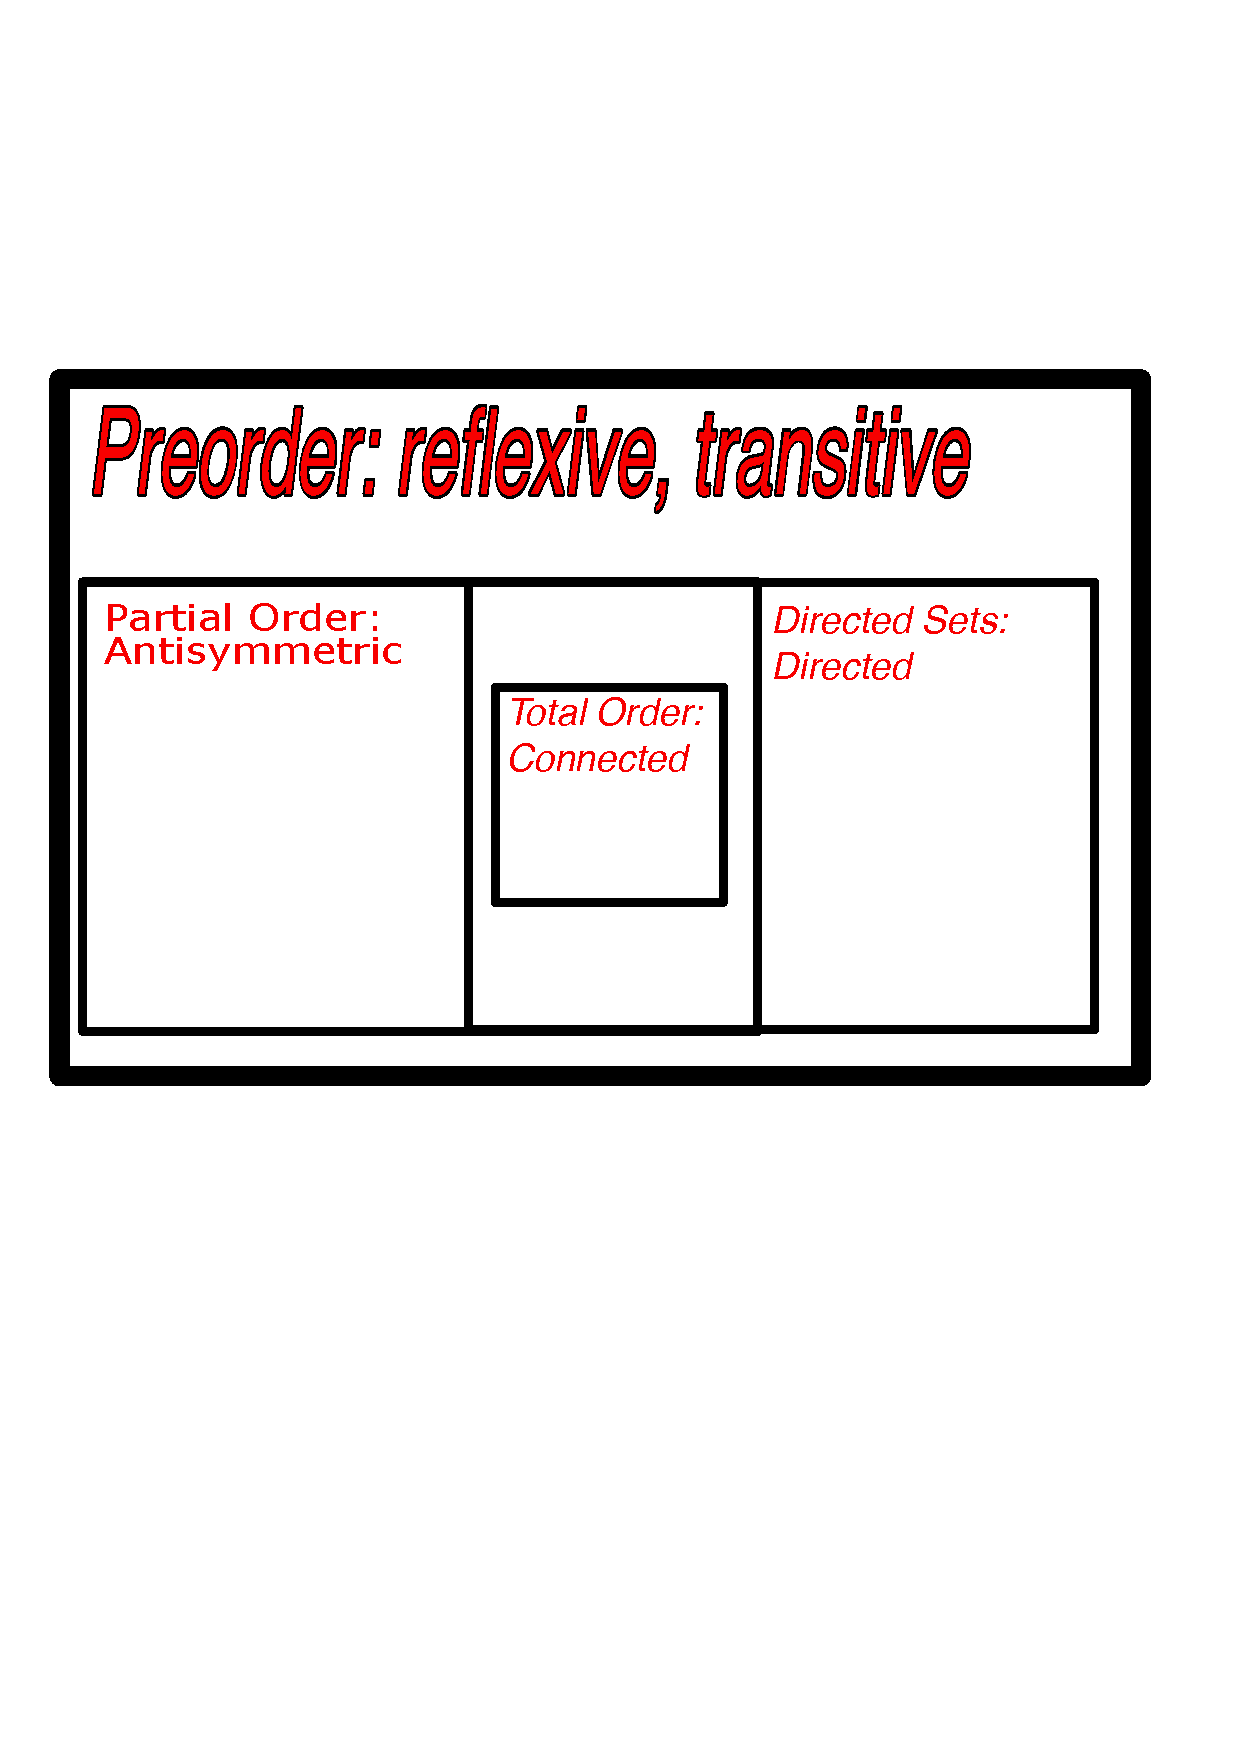
\includegraphics[height=10cm,width=10cm]{drawing.pdf}
\end{mdframed}
\begin{definition}
\label{1.1.9}
\textbf{(Definition of Cofinal)} Given a directed set $\mathcal{D}$, a subset $\mathcal{D}'\subseteq \mathcal{D}$ is called cofinal if 
\begin{align*}
\forall d \in \mathcal{D},\exists e\in \mathcal{D}', d\leq e 
\end{align*}
\end{definition}
\begin{theorem}
\label{1.1.10}
\textbf{(Cofinal Subset is a Directed Set with Original Order)} Given a directed set $\mathcal{D}$
 \begin{align*}
 \mathcal{D}'\subseteq \mathcal{D}\text{ is cofinal }\implies \mathcal{D}'\text{ is a directed set }
 \end{align*}
\end{theorem}
\begin{proof}
Arbitrarily pick two $a,b \in \mathcal{D}'$. Because $\mathcal{D}\ni a,b$ is directed, we know 
\begin{align*}
\exists c \in \mathcal{D}, a\leq c \text{ and } b\leq c
\end{align*}
Then because $\mathcal{D}'$ is cofinal in $\mathcal{D}$, we know 
\begin{align*}
\exists d \in \mathcal{D}', c\leq d
\end{align*}
Then because transitivity of directed set, our proof is finished, as we have found an element $d$ in $\mathcal{D}'$ that is greater than the arbitrary picked elements $a,b \in \mathcal{D}'$. 
\end{proof}
\section{Net}
\begin{definition}
\label{1.2.1}
  \textbf{(Subnet)} Given a net $w:\mathcal{D}\rightarrow X$ and $v:\mathcal{E}\rightarrow X$ and a function $h:\mathcal{E}\rightarrow \mathcal{D}$ we say $v$ is a subnet of $w$ if  
\begin{align*}
\begin{cases}
\forall e,e' \in \mathcal{E}, e\leq e' \implies h(e)\leq h(e')\text{(monotone)}\\
h[E]\text{ is cofinal in $\mathcal{D}$ }\\
v=w\circ h
\end{cases}
\end{align*}
\end{definition}
\begin{definition}
\textbf{(Net convergence)} We say the net $w:\mathcal{D}\rightarrow X$ converge to $x$, $w \to x$ if 
\begin{align*}

\end{align*}
\end{definition}
\begin{theorem}
\textbf{($w \to x \implies v \to x$)} Suppose $v$ is a subnet of $w$, we have 
 \begin{align*}
w \to x \implies v \to x
\end{align*}
\end{theorem}
\begin{proof}

\end{proof}
\begin{theorem}
\textbf{()}
\end{theorem}
\begin{definition}
\textbf{()}
\end{definition}
\chapter{Metric Space}
\section{}      
\chapter{Calculus}
\section{Examples for uniform convergence} 
\begin{theorem}
\textbf{(Test Example)} The sequence 
\begin{align*}
f_n(x)=\frac{x^2}{x^2+(1-nx)^2}\text{ is not equicontinuous on $[0,1]$ }
\end{align*}
\end{theorem}
\begin{proof}
Notice that 
\begin{align*}
f_n(\frac{1}{n})=1\text{ and }f_n(0)=0
\end{align*}
Then for all $\delta$, we see that if $n$ is large enough 
 \begin{align*}
\text{ then }\abso{\frac{1}{n}-0}<\delta \text{ and }\abso{f_n(\frac{1}{n})-f_n(0)}=1
\end{align*}
\end{proof}
\begin{theorem}
\textbf{(Test Example)} Prove 
\begin{align*}
\frac{x}{1+nx^2}\text{ uniformly converge on $\R$ }
\end{align*}
\end{theorem}
\begin{proof}
It is clear that $\frac{x}{1+nx^2}$ pointwise converge to $0$. Because $\frac{x}{1+nx^2}$ is an odd function, fixing $\epsilon $, we only wish to find $N$ such that 
\begin{align*}
\forall x>0, \forall n>N, \frac{x}{1+nx^2}<\epsilon 
\end{align*}
Observe 
\begin{align*}
  \frac{x}{1+nx^2}<\epsilon &\iff x<\epsilon (1+nx^2)\\
  &\iff \frac{x-\epsilon }{\epsilon x^2}<n
\end{align*}
Notice that $\frac{x-\epsilon }{\epsilon x^2}$ is bounded since it is continuous and converge to $0$ as  $x \to \infty$. 
\end{proof}
\section{Test Example}
\begin{theorem}
\textbf{(Cauchy-Schwarz Inequality for Integral)} Let $\mathscr{R}\Big([a,b] \Big)$ be the space of Riemann-Integrable functions on $[a,b]$. It is clear that $\mathscr{R}\Big([a,b] \Big)$ is a vector space over $\R$.  Define $\langle \cdot , \cdot \rangle $ on $\mathscr{R}\Big([a,b] \Big)$ by 
\begin{align*}
\langle f,g\rangle = \int_a^b f(x)g(x)dx
\end{align*}
It is easy to show  
\begin{enumerate}[label=(\alph*)]
  \item $ \forall f \in \mathscr{R}\Big([a,b] \Big), \langle f,f\rangle \geq 0 $ (non-negativity) 
  \item $\forall f,g \in \mathscr{R}\Big([a,b] \Big),\langle f,g\rangle =\langle g,f\rangle $ (Symmetry)
  \item $\forall f,g,h \in \mathscr{R}\Big([a,b] \Big),\forall c \in \R, \langle cf+g,h\rangle =c\langle f,h\rangle +\langle g,h \rangle $ (Linearity in first argument)
\end{enumerate}
This make $\langle \cdot,\cdot\rangle $ a \textbf{positive semi-definite Hermitian form}. We shall prove Cauchy-Schwarz Inequality hold for positive semi-definite Hermitian form. That is, we shall prove 
\begin{align*}
\forall f ,g \in \mathscr{R}\Big([a,b] \Big),\langle f,g \rangle \leq \norm{f}\cdot \norm{g}
\end{align*}
\end{theorem}
\begin{proof}
\end{proof}
\begin{theorem}
\textbf{(Application)} Given $f \in \mathscr{R}\Big([a,b] \Big)$ such that 
\begin{enumerate}[label=(\alph*)]
  \item $f(a)=0=f(b)$ 
  \item $\int_a^b f^2 (x)dx =1$ 
  \item $f$ is continuously differentiable on  $(a,b)$
  \item $f' \in \mathscr{R}\Big([a,b] \Big)$
\end{enumerate}
We have 
\begin{align*}
\int_a^b xf(x)f'(x)=\frac{-1}{2}
\end{align*}
and have 
\begin{align*}
\int_a^b \big(f'(x) \big)^2 dx \cdot \int_a^b \big(xf(x) \big)^2 dx>\frac{1}{4}
\end{align*}


\end{theorem}
\begin{proof}
Notice that 
\begin{align*}
  \frac{d}{dx} xf^2(x)=f^2(x)+2xf(x)f'(x)
\end{align*}
Then by Integral by Part (We have to check $\big(xf^2(x) \big)'(t)=f^2(t)+2tf(t)f'(t)$ for all $t \in (a,b)$, and we have to check $xf^2(x)$ is continuous on $[a,b]$), we have 
\begin{align*}
1=\int_a^b f^2(x)dx=xf^2(x)\Big|_a^b - \int_a^b 2xf(x)f'(x)dx
\end{align*}
Then because $f(b)=f(a)=0$, we see 
\begin{align*}
2 \int_a^b xf(x)f'(x)dx=-1 
\end{align*}
We wish to show 
\begin{align*}
\norm{f'}^2 \cdot \norm{x f(x)}^2> \frac{1}{4}= \Big( \langle f',xf(x)\rangle \Big)^2
\end{align*}
It is clear that $\geq $ is valid from Cauchy-Schwarz Inequality. We have to prove $\neq $. In other words, we have to prove 
\begin{align*}
f'\text{ and }xf(x)\text{ are linearly independent }
\end{align*}
\As{$f'$ and $xf(x)$ are linearly dependent}. Then 
 \begin{align*}
\exists c\inr, \forall x\in [a,b], f'(x)=cxf(x)
\end{align*}
The solution for this first order linear homogeneous ODE is 
\begin{align*}
f(x)=Ae^{\frac{cx^2}{2}} \text{ where $A\inr$ depends on $f(a)$ and $f(b)$}
\end{align*}
Then because $f(a)=f(b)=0$, we see $A=0$. Then  $\int_a^b f^2(x)dx=0\tCaC$
\end{proof}
\begin{theorem}
\textbf{(Example)} Given $G,g,\alpha :[a,b]\rightarrow \R$, suppose
\begin{enumerate}[label=(\alph*)]
  \item $G'(x)=g(x)$ for all $x \in (a,b)$ ($G$ is differentiable  on  $(a,b)$)
  \item $G$ is continuous on  $[a,b]$
  \item $\alpha $ increase on $[a,b]$
  \item $g$ is properly Riemann-Integrable on  $[a,b]$
\end{enumerate}
Prove 
\begin{align*}
\int_a^b \alpha (x)g(x)dx= \alpha G\Big|_a^b - \int_a^b G(x)d\alpha  
\end{align*}
\end{theorem}
\begin{proof}

\end{proof}
\section{Dini's Theroem}
\begin{theorem}
\textbf{(Dini's Theorem)} Given a topological space $X$ and a sequence of functions  $f_n:X\rightarrow \R$, suppose
\begin{enumerate}[label=(\alph*)]
  \item $X$ is compact
  \item $f_n$ is continuous  
  \item $f_n\to f$ pointwise  
  \item $f$ is continuous  
  \item $f_n(x)\leq f_{n+1}(x)$ for all $x \in X$
\end{enumerate}
Then 
\begin{align*}
f_n \to f \text{ uniformly }
\end{align*}
\end{theorem}
\begin{proof}
  Define $g_n:X\rightarrow \R$ 
\begin{align*}
g_n=f-f_n
\end{align*}
We reduce the problem into 
\begin{align*}
\vi{\text{ proving }g_n \to 0\text{ uniformly }}
\end{align*}
Notice that we have the property 
\begin{enumerate}[label=(\alph*)]
  \item $g_n(x)\geq g_{n+1}(x)$ for all $x \in X$ 
  \item $g_n$ is continuous 
   \item $g_n \to 0$ pointwise
\end{enumerate}
Fix $\epsilon $. We wish 
\begin{align*}
\vi{\text{ to find $N$ such that }\forall n>N, \forall x \in X,  g_n(x)<\epsilon }
\end{align*}
Define $E_n \subseteq X$ by 
\begin{align*}
E_n= \set{x \in X: g_n(x)<\epsilon }
\end{align*}
Because $g_n$ is continuous and  $E_n=g_n^{-1}\Big[(-\infty,\epsilon ) \Big]$, we know 
\begin{align*}
E_n\text{ is open for all $n \inn$ }
\end{align*}
We first prove 
\begin{align*}
\blue{\set{E_n}_{n\inn}\text{ is an open cover of $X$ }}
\end{align*}
Fix $y \in X$. We wish 
\begin{align*}
\blue{\text{ to find $n$ such that }y \in E_n}
\end{align*}
Because $g_n(y)\to 0$, this is clear. $\bdone$\\

We now prove 
\begin{align*}
\olive{\set{E_n}_{n\inn}\text{ is ascending }}
\end{align*}
Fix $n \inn$. We wish 
\begin{align*}
\olive{\text{ to prove }E_n\subseteq E_{n+1}}
\end{align*}
Because $g_n(x)\geq g_{n+1}(x)$ for all $x \in X$ and $E_n=g_{n}^{-1}\Big[(-\infty,\epsilon ) \Big]$ by definition, we see 
\begin{align*}
y \in E_n \implies g_{n+1}(y)<g_n(y)<\epsilon \implies y \in E_{n+1}\odone
\end{align*}
Now, because $X$ is compact and $\set{E_n}_{n\inn}$ is an open cover of $X$, we know  
\begin{align}
\label{Dimi1}
\text{ there exists $N$ such that  $X \subseteq \bigcup_{k=1}^N E_k= E_N$ }
\end{align}
It is clear such $N$ works.  $\vdone$
\end{proof}



\chapter{Multi-Variable Calculus}
\section{}
\end{document}
